\section{Descrição do Problema e Complexidade}

Seja $G=(V,E)$ um grafo não direcionado com $n=|V|$ vértices e $m=|E|$ arestas, em que cada aresta $uv$ tem um peso inteiro $w_{uv}$. Uma partição é uma função $s:V\to\{0,1\}$, e o valor do corte é
\begin{equation}
  \mathrm{cut}(s)=\sum_{uv\in E,\; s(u)\neq s(v)} w_{uv}.
\end{equation}
O problema pede uma partição de valor máximo, $\mathrm{OPT}=\max_s \mathrm{cut}(s)$. Usamos a mesma notação do Trabalho~1: $N(v)$ é a vizinhança de $v$, $\Delta$ é o grau máximo e $W=\sum_{uv\in E}|w_{uv}|$.

\subsection{Complexidade}

A versão de decisão (existe um corte de valor pelo menos $k$?) está em NP, pois uma partição é verificada em $O(n+m)$, e é NP-completa \cite{Karp 1972, Garey et al. 1976}. Logo a versão de otimização é NP-difícil e não se espera um algoritmo polinomial exato, a menos que P $=$ NP. Todo algoritmo exato conhecido para o caso geral leva tempo exponencial. A enumeração das $2^{n-1}$ partições (a menos de simetria) resolve o problema em tempo $O(2^n)$ com código de Gray, e o melhor limite de pior caso que conhecemos é o de \citet{Williams 2005}, de ordem $O(2^{\omega n/3})$ ($\omega$ é o expoente da multiplicação de matrizes), cerca de $1{,}73^n$, mas ao custo de memória também exponencial e sem utilidade prática em grafos esparsos.

Há casos tratáveis. Em grafos planares o problema é polinomial \cite{Hadlock 1975}, o que inclui as grades com contorno periódico em no máximo uma direção \cite{Liers et al. 2003}; o toro, periódico nas duas direções, que é a classe das nossas grades, não é planar. Em grafos de largura de caminho (ou de árvore) $w$, programação dinâmica resolve o problema em tempo $O(2^{w}\cdot \mathrm{poly}(n))$ \cite{Arnborg et al. 1991, Bodlaender 1993}, o que é a base do segundo algoritmo deste trabalho. Os dois extremos explicam a escolha de instâncias: o problema é tratável quando o grafo tem estrutura (largura pequena) e difícil quando não tem (grafos aleatórios), embora esparsos.

\section{Estado da Arte em Algoritmos Exatos}

Os métodos exatos práticos para o Max-Cut dividem-se em três famílias.

\paragraph{Branch-and-cut poliédrico.} Formulam o problema como programação linear sobre o politopo de corte e acrescentam desigualdades válidas (de ciclo ímpar, de triângulo, entre outras) durante a busca. \citet{Barahona et al. 1988} aplicaram essa abordagem a estados fundamentais de vidros de spin e ao projeto de circuitos, e \citet{Liers et al. 2004} descrevem o seu uso para vidros de spin difíceis. \citet{Liers et al. 2003} calcularam os estados fundamentais de vidros de spin em grafos aleatórios regulares de grau 4 e 6 (acoplamentos gaussianos) com até 1\,280 spins, uma classe próxima dos nossos grafos aleatórios esparsos ($m=2n$ tem grau médio 4), e observaram que o tempo cresce de forma polinomial na fase ferromagnética e mais que polinomial na fase de vidro de spin. Métodos poliédricos são, em geral, os mais indicados para grafos esparsos.

\paragraph{Branch-and-bound semidefinido.} Calculam os limitantes com a relaxação semidefinida do problema reforçada por desigualdades de triângulo. O \emph{Biq Mac} \cite{Rendl et al. 2010} resolve em tempo razoável qualquer instância de até $n=100$ vértices, qualquer que seja a densidade, e é o método de referência para grafos densos; os próprios autores observam que, para grafos esparsos, métodos baseados em programação linear podem ser preferíveis. \citet{Krislock et al. 2014} melhoraram o cálculo dos limitantes e relatam desempenho superior ao do Biq Mac na maior parte das instâncias testadas.

\paragraph{Exploração de estrutura.} Para grafos de largura de caminho ou de árvore pequena, a programação dinâmica sobre a decomposição é exata e de custo $O(2^{w}\mathrm{poly}(n))$ \cite{Arnborg et al. 1991, Bodlaender 1993}. A largura de caminho é igual ao número de separação de vértices de um melhor ordenamento \cite{Kinnersley 1992}, o que permite implementá-la como um percurso por uma ordem de vértices, como fazemos na Seção~5.2.

Nossos dois algoritmos ocupam posições modestas nesse panorama. O Branch-and-Bound usa um limitante barato, calculado em $O(\deg v)$ por nó, em vez de relaxações lineares ou semidefinidas; ele troca qualidade do limitante por velocidade por nó. A programação dinâmica é a versão mais simples da terceira família. Não esperamos competir com \emph{Biq Mac} ou com os resolvedores de branch-and-cut, e a comparação com a literatura da Seção~7 deve ser lida com esse cuidado.

\section{Técnicas Escolhidas}

\paragraph{Branch-and-Bound.} Constrói a partição vértice a vértice, ramificando nos dois lados possíveis, e poda um ramo quando um limitante superior do valor de qualquer completação não supera o melhor corte já conhecido. Não exige nenhuma estrutura do grafo e funciona com pesos de qualquer sinal; sua eficiência depende só da qualidade do limitante e da ordem de decisão. Usamos como limite inferior inicial a heurística do Trabalho~1, o que liga os dois trabalhos: uma heurística boa poda mais desde o primeiro nó.

\paragraph{Programação dinâmica sobre a fronteira.} Processa os vértices em uma ordem fixa e mantém, para cada atribuição possível dos vértices da \emph{fronteira} (processados que ainda têm vizinhos por processar), o melhor valor parcial. Quando um vértice perde o último vizinho pendente, ele sai da fronteira e o algoritmo maximiza sobre o seu lado. A Figura~\ref{fig:fronteira} ilustra o percurso. O custo é exponencial apenas na largura da fronteira, e não em $n$.

As duas técnicas são complementares. O Branch-and-Bound é geral, mas seu tempo explode com $n$ mesmo em grafos esparsos. A programação dinâmica depende da estrutura, mas, quando ela existe, resolve instâncias com milhares de vértices. Como o tema do Trabalho~1 foi grafos grandes e esparsos, a segunda técnica é a mais natural para o contraste com a heurística.

\begin{figure}[ht]
\centering
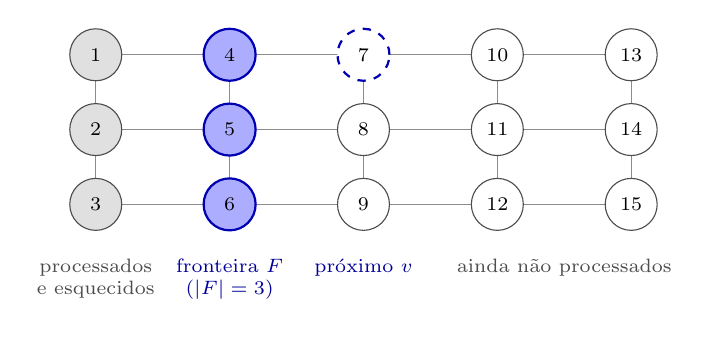
\begin{tikzpicture}[x=1.7cm,y=-0.95cm,
  vtx/.style={circle,draw=black!70,minimum size=0.66cm,inner sep=0pt,font=\scriptsize},
  proc/.style={vtx,fill=black!12},
  fron/.style={vtx,fill=blue!32,draw=blue!70!black,thick},
  prox/.style={vtx,fill=white,draw=blue!70!black,thick,dashed},
  nao/.style={vtx,fill=white},
  aresta/.style={draw=black!45}]
  \foreach \c in {1,...,5}{\foreach \r in {1,2,3}{
    \pgfmathtruncatemacro{\id}{(\c-1)*3+\r}
    \coordinate (p\c\r) at (\c,\r);
  }}
  \foreach \c in {1,...,5}{\foreach \r in {1,2,3}{
    \pgfmathtruncatemacro{\cc}{\c+1}\pgfmathtruncatemacro{\rr}{\r+1}
    \ifnum\c<5 \draw[aresta] (p\c\r) -- (p\cc\r); \fi
    \ifnum\r<3 \draw[aresta] (p\c\r) -- (p\c\rr); \fi
  }}
  \foreach \c/\sty in {1/proc,2/fron,3/nao,4/nao,5/nao}{\foreach \r in {1,2,3}{
    \pgfmathtruncatemacro{\id}{(\c-1)*3+\r}
    \ifnum\c=3\ifnum\r=1 \node[prox] at (p\c\r) {\id}; \else \node[nao] at (p\c\r) {\id}; \fi
    \else \node[\sty] at (p\c\r) {\id}; \fi
  }}
  \node[anchor=north,align=center,font=\scriptsize,text=black!70] at (1,3.6) {processados\\e esquecidos};
  \node[anchor=north,align=center,font=\scriptsize,text=blue!60!black] at (2,3.6) {fronteira $F$\\($|F|=3$)};
  \node[anchor=north,align=center,font=\scriptsize,text=blue!60!black] at (3,3.6) {próximo $v$};
  \node[anchor=north,align=center,font=\scriptsize,text=black!70] at (4.5,3.6) {ainda não processados};
\end{tikzpicture}
\caption{Percurso da programação dinâmica em uma grade $3\times5$ numerada por colunas. Os vértices 1 a 3 já saíram da fronteira (todos os seus vizinhos foram processados); os vértices 4 a 6 formam a fronteira $F$, porque cada um ainda tem vizinho na coluna seguinte. Ao inserir o vértice 7, a tabela tem $2^{|F|+1}=16$ entradas.}\label{fig:fronteira}
\end{figure}

\section{Algoritmos Implementados}

\subsection{Algoritmo 1: Branch-and-Bound}

Os vértices são decididos em uma ordem $\pi$ calculada de forma gulosa: começa-se pelo vértice de maior peso ponderado $\sum|w|$, e o próximo é sempre o que tem maior peso $|w|$ total para os já ordenados. Assim as arestas ficam ``decididas'' (as duas pontas fixadas) o mais cedo possível e o limitante se torna justo cedo. Quando o próximo vértice não tem nenhum vizinho já ordenado, ele abre uma nova componente conexa.

Em um nó da busca, os vértices $\pi_1,\dots,\pi_{i}$ estão decididos. Para cada vértice $v$ ainda não decidido mantemos $c_0(v)$ e $c_1(v)$, os pesos das arestas de $v$ para vizinhos já decididos nos lados 0 e 1. Colocar $v$ no lado $s$ corta exatamente as arestas para decididos do lado oposto, com ganho $c_{1-s}(v)$. Seja $\mathrm{cut}_\sigma$ o valor das arestas já decididas que estão cortadas. O limitante superior é
\begin{equation}\label{eq:ub}
  \mathrm{UB}(\sigma)=\mathrm{cut}_\sigma+\sum_{v\ \text{livre}}\max\{c_0(v),c_1(v)\}+\sum_{\substack{uv\in E\\ u,v\ \text{livres}}}\max\{w_{uv},0\}.
\end{equation}

\begin{lema}\label{lema:ub}
Para toda completação $s$ da solução parcial $\sigma$, $\mathrm{cut}(s)\le \mathrm{UB}(\sigma)$.
\end{lema}
\begin{prova}
Separe as arestas em três classes. As que têm as duas pontas decididas contribuem exatamente $\mathrm{cut}_\sigma$, qualquer que seja a completação. Uma aresta $uv$ com $v$ livre e $u$ decidido só é cortada se $v$ ficar do lado oposto de $u$; assim, o que as arestas de $v$ para decididos contribuem é $c_{1-s(v)}(v)\le\max\{c_0(v),c_1(v)\}$. Por fim, uma aresta entre dois livres contribui $w_{uv}$ ou $0$, no máximo $\max\{w_{uv},0\}$. Somando as três classes, obtém-se (\ref{eq:ub}). \qed
\end{prova}

As três parcelas de (\ref{eq:ub}) são mantidas de forma incremental: ao fixar $v$ no lado $s$, só mudam as parcelas de $v$ e de seus vizinhos livres, em tempo $O(\deg v)$, e o desfazer é simétrico. O algoritmo ramifica primeiro no lado que corta mais peso (o de maior ganho), pois isso tende a encontrar boas soluções cedo. Como o valor de uma partição não muda ao trocar os dois lados de uma componente inteira, o primeiro vértice de cada componente é fixado no lado 0, o que corta a busca pela metade por componente. O Algoritmo~\ref{alg:bb} resume o procedimento.

\begin{algorithm}[ht]
\caption{Branch-and-Bound}\label{alg:bb}
\begin{algorithmic}[1]
\Require grafo $G=(V,E,w)$, tempo máximo $T$
\Ensure partição $s^*$ de valor máximo (ou a melhor encontrada, se o tempo acabar)
\State $s^*\gets$ heurística do Trabalho 1; \quad $\mathit{melhor}\gets \mathrm{cut}(s^*)$
\State calcular a ordem $\pi$ e inicializar $c_0,c_1,\mathrm{cut}_\sigma,\mathrm{UB}$
\Procedure{Rec}{$i$}
  \If{$\mathrm{UB}(\sigma)\le \mathit{melhor}$} \State \textbf{retornar} \Comment{poda}
  \EndIf
  \If{$i=n$} \State $\mathit{melhor}\gets \mathrm{cut}_\sigma$; \quad $s^*\gets\sigma$; \quad \textbf{retornar}
  \EndIf
  \State $v\gets\pi_i$
  \For{$s\in\{0,1\}$, começando pelo lado de maior ganho \textbf{e pulando} $s=1$ se $v$ abre componente}
    \State fixar $v$ no lado $s$; \quad \Call{Rec}{$i+1$}; \quad desfazer
  \EndFor
\EndProcedure
\State \Call{Rec}{$0$}; \quad \textbf{devolva} $s^*$
\end{algorithmic}
\end{algorithm}

\begin{teorema}[Correção]\label{teo:bb}
Se o Algoritmo~\ref{alg:bb} termina sem estourar o tempo, $\mathrm{cut}(s^*)=\mathrm{OPT}$.
\end{teorema}
\begin{prova}
O valor $\mathit{melhor}$ é sempre o corte de uma partição válida ($s^*$), pois começa com a da heurística e só é atualizado em folhas, onde $\mathrm{UB}=\mathrm{cut}$. Suponha, por contradição, que exista $s'$ com $\mathrm{cut}(s')>\mathit{melhor}$ ao final. Pela simetria por componente, podemos supor que $s'$ tem lado 0 no primeiro vértice de cada componente, pois trocar todos os lados de uma componente preserva o valor do corte e não cria nem remove arestas cortadas entre componentes (não há arestas entre elas). Então $s'$ é uma folha da árvore completa de decisões. Em todo nó $\sigma$ do caminho até $s'$, o Lema~\ref{lema:ub} dá $\mathrm{UB}(\sigma)\ge\mathrm{cut}(s')>\mathit{melhor}_{\text{final}}$, e como $\mathit{melhor}$ só cresce, $\mathrm{UB}(\sigma)>\mathit{melhor}$ no momento da visita. Logo nenhum nó do caminho é podado, a folha $s'$ é visitada, e nela $\mathrm{cut}(s')>\mathit{melhor}$ faz o algoritmo atualizar $\mathit{melhor}$ para pelo menos $\mathrm{cut}(s')$, o que contradiz $\mathit{melhor}_{\text{final}}<\mathrm{cut}(s')$. \qed
\end{prova}

\paragraph{Complexidade.} Cada nó custa $O(\deg v)$, e a árvore tem no máximo $2^{n-c+1}$ nós ($c$ componentes), então o pior caso é $O(2^{n}\,\Delta)$ em tempo e $O(n+m)$ em memória. Não há garantia melhor: o limitante \eqref{eq:ub} é fraco quando a maior parte do peso fica em arestas entre vértices livres, de modo que o número de nós visitados cresce exponencialmente com $n$ na prática também, como mostra a Seção~7.

\subsection{Algoritmo 2: Programação dinâmica sobre a fronteira}

Dada uma ordem $\pi=(v_1,\dots,v_n)$, seja $P_i=\{v_1,\dots,v_i\}$ o conjunto dos $i$ primeiros vértices e
\[F_i=\{u\in P_i : u \text{ tem algum vizinho fora de } P_i\}\]
a \emph{fronteira}. Para $x\in\{0,1\}^{F_i}$, defina
\begin{equation}
  f_i(x)=\max\Big\{\sum_{\substack{uv\in E,\ u,v\in P_i\\ y_u\ne y_v}} w_{uv}\ :\ y\in\{0,1\}^{P_i},\ y|_{F_i}=x\Big\},
\end{equation}
o melhor valor, entre as arestas já completamente processadas, de uma atribuição que concorda com $x$ na fronteira. Temos $F_0=\emptyset$ e $f_0(\emptyset)=0$. O passo $i$ tem duas fases.

\emph{Inserção.} Os vizinhos de $v_i$ em $P_{i-1}$ pertencem todos a $F_{i-1}$, pois cada um tem $v_i$ como vizinho ainda não processado. Logo o ganho de colocar $v_i$ no lado $s$ depende só de $x$:
\begin{equation}
  h(x,s)=f_{i-1}(x)+\sum_{u\in N(v_i)\cap F_{i-1},\ x_u\ne s} w_{uv_i},\qquad x\in\{0,1\}^{F_{i-1}},\ s\in\{0,1\}.
\end{equation}
Se a fronteira está vazia, $v_i$ abre uma componente nova e fixamos $s=0$ (simetria). A tabela passa a ter $2^{|F_{i-1}|+1}$ entradas.

\emph{Esquecimento.} Todo $u$ na tabela que não tem mais vizinhos fora de $P_i$ é eliminado, por maximização sobre o seu lado: $f(x_{-u})=\max_{b\in\{0,1\}} h(x_{-u},x_u{=}b)$. O algoritmo guarda um bit por estado dizendo qual $b$ venceu. Ao final, $F_n=\emptyset$ e $f_n(\emptyset)=\mathrm{OPT}$. A partição ótima é recuperada percorrendo os passos em ordem inversa: em cada esquecimento, o bit guardado dá o lado do vértice eliminado.

\begin{teorema}[Correção]\label{teo:dp}
Para toda ordem $\pi$, a tabela $f_n$ calculada pelo algoritmo satisfaz $f_n(\emptyset)=\mathrm{OPT}$, e a partição reconstruída tem corte $\mathrm{OPT}$.
\end{teorema}
\begin{prova}
Por indução em $i$, mostramos que a tabela calculada coincide com $f_i$. A base é trivial. No passo de inserção, uma atribuição $y$ de $P_i$ é a de $P_{i-1}$ mais o lado $s$ de $v_i$; as arestas novas são as que ligam $v_i$ a $P_{i-1}$, todas com a outra ponta em $F_{i-1}$, e o seu valor depende só de $y|_{F_{i-1}}=x$ e de $s$, o que dá $h$. Maximizar sobre as atribuições de $P_{i-1}$ compatíveis com $x$ resulta em $f_{i-1}(x)+\text{ganho}(x,s)$. No esquecimento, um vértice $u$ eliminado não tem mais arestas para vértices não processados, então nenhuma aresta futura depende de $y_u$, e a maximização sobre $y_u$ não perde nenhuma completação. Para $i=n$ a fronteira é vazia e $f_n(\emptyset)$ é o máximo sobre todas as atribuições, que é $\mathrm{OPT}$. A restrição $s=0$ ao abrir componente não perde o ótimo, pelo mesmo argumento de simetria do Teorema~\ref{teo:bb}. A reconstrução desfaz as maximizações na ordem inversa, e o bit guardado em cada estado é o que realizou o máximo, logo a partição obtida atinge $f_n(\emptyset)$. \qed
\end{prova}

\paragraph{Complexidade.} Seja $w=\max_i(|F_{i-1}|+1)$, o tamanho em bits da maior tabela. A inserção do vértice $v_i$ percorre $2^{|F_{i-1}|}$ estados, cada um em $O(\deg^-(v_i))$ (vizinhos já processados); cada esquecimento custa $O(2^{w-1})$ e há $n$ no total. O tempo é $O(n\,2^{w}+2^{w}\,m)=O(2^{w}(n+m))$, e a memória, $O(2^{w})$ para duas tabelas mais $O(n\,2^{w})$ \emph{bits} para os ponteiros de reconstrução. O valor $w-1$ é o número de separação de vértices da ordem, e o mínimo sobre todas as ordens é a largura de caminho do grafo \cite{Kinnersley 1992}; portanto, com a melhor ordem, o tempo é $O(2^{\mathrm{pw}(G)+1}(n+m))$. Achar a melhor ordem é difícil; usamos a heurística descrita a seguir.

\paragraph{Escolha da ordem.} Um guloso que, a cada passo, escolhe entre os vértices adjacentes à fronteira aquele que minimiza o tamanho da fronteira resultante (desempate pelo menor número de vizinhos pendentes e, depois, ao acaso). A construção é repetida a partir de até 30 vértices iniciais diferentes (o primeiro, de menor grau) e fica-se com a ordem de menor $w$. Antes de alocar qualquer tabela, o programa simula a ordem para conhecer $w$ e a memória necessária e recusa a execução se $w>26$ (parâmetro) ou se a memória passar de 2\,GB. A Figura~\ref{fig:fronteira} mostra uma ordem que varre a grade pelo lado longo; é o que o guloso aparenta encontrar nas grades toroidais (fronteira de $2L$ vértices mais o vértice inserido, ou seja, $w=2L+1$, como se vê na Tabela~\ref{tab:principal}).

